\documentclass{beamer}
\usepackage{tikz-cd}
\usetheme{Boadilla}

\title{Objective Description in Physics}
\subtitle{What is it?  What good is it?}
\author{Hans Halvorson}
\institute{Princeton University}
\date{August 9, 2019}


\begin{document}

\begin{frame}
\titlepage
\end{frame}

\begin{frame}

\begin{itemize}
\item Objectivity as a concrete scientific virtue
\item The demand for objectivity as a norm for choosing research paradigms
\item In public discussion, the sciences (and esp physics) are taken
  as the paradigm of objectivity
\item Two pictures of objectivity: Einstein (mind of god) versus Bohr
  (unambiguous communication)
\end{itemize}


\end{frame}

\begin{frame}
\frametitle{Outline}
\tableofcontents
\end{frame}

\section{Einstein's divine aspiration}

\begin{frame}

  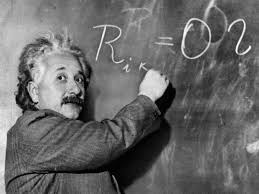
\includegraphics[scale=0.7]{einstein.jpeg}

  ``I want to know God's thoughts, the rest are details.''

\end{frame}

\begin{frame}
  \frametitle{Bernard Williams: the absolute conception}

  \begin{figure}[r] 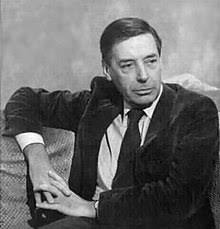
\includegraphics[scale=0.3]{williams.jpeg} \end{figure}

``What God has given us, according to Descartes, is an insight into
the nature of \underline{the world as it seems to God}, and the world
as it seems to God must be the world as it really is.'' (p 196)

\bigskip \bigskip ``\dots a conception of reality as it is
\underline{independently of our thought}, and to which all
representations of reality can be related.''  (p 196)

\bigskip \bigskip ``If what they both have is knowledge, then it seems
to follow that there must be some coherent way of understanding why
these representations differ, and how they are related to one
another.'' (p 49)
\end{frame}

\begin{frame}
  \frametitle{North Atlantic Metaphysical Madness \\ theory without convention}

  \begin{tabular}{c c c}
    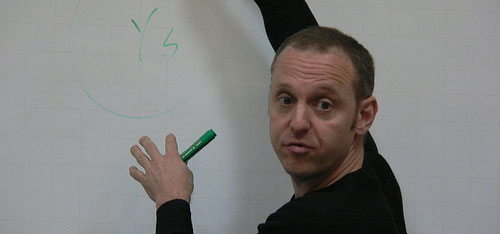
\includegraphics[scale=0.25]{sider.jpg} &
                                              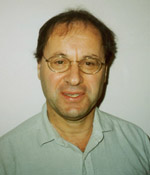
\includegraphics[scale=1.5]{find.jpg}
    & 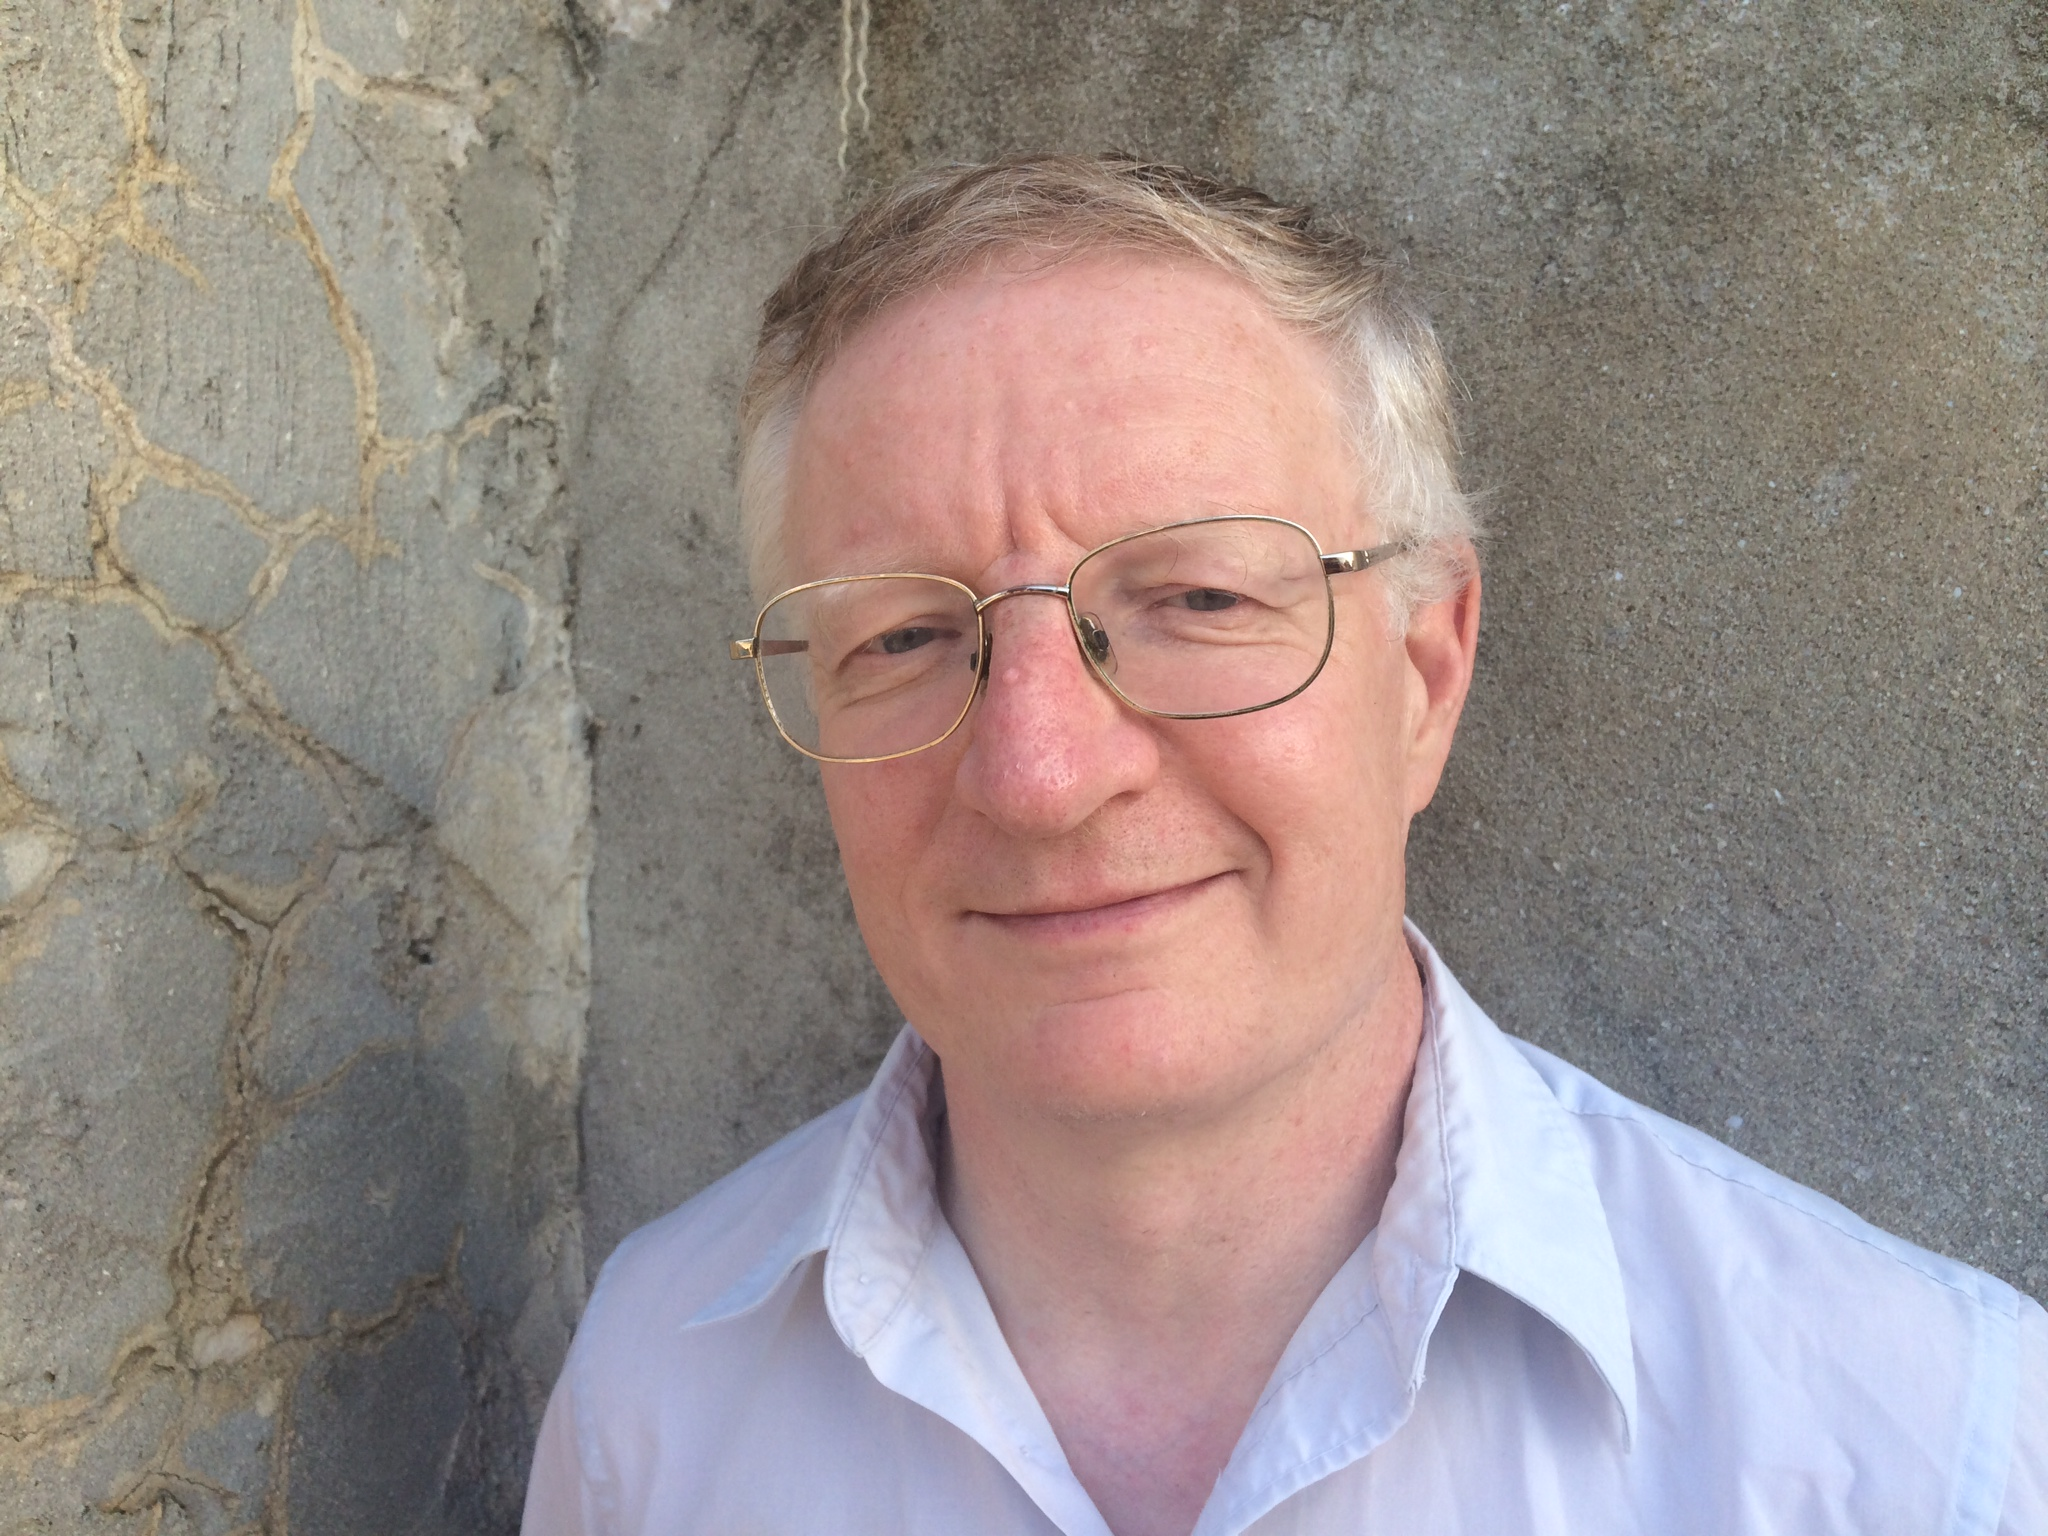
\includegraphics[scale=0.04]{williamson.jpg} \end{tabular}

  %% TO DO: pictures of Sider, Fine, Williamson

  %% TO DO: tikz picture with arrows

\bigskip
                                            
  \begin{tabular}{l l l l l}
    $T_1$ & & $\forall x\exists yRxy$  & & \\ \\
    $T_2$ & & $\forall y\exists xRxy$ \\ \\
    $T^+$ & & there is a serial relation \end{tabular}

  %% TO DO: picture of the common definitional extension


  \end{frame}
\begin{frame}
  \frametitle{coordinate free description}

%% affine space as CDE

\end{frame}

\begin{frame}
  \frametitle{science liberated from language}

  ``The semantic view of theories makes language irrelevant to the
  subject'' (Bas van Fraassen)

  \bigskip ``In our discussion, a model is not such an interpretation [i.e.,
  not an $\Sigma$-structure], matching statements to a set of objects
  which bear certain relations among themselves, but the set of
  objects itself.'' (Lisa Lloyd)

\bigskip   \[ \{ \{ a,b,\langle a,a\rangle \} , \{ \langle a,a\rangle \} \} \]
  
  %% Lisa Lloyd

 \end{frame}

\begin{frame}
\frametitle{Summary: the Einstein view of objectivity}
  
  \begin{enumerate}
  \item The absolute conception (Williams) / view from nowhere (Nagel)
    / god's eye view (Putnam)
  \item Theory without conventions
  \item Spacetime description without coordinates
  \item Theory without language
    \newline
    No need for coordinative definitions
    \item Perfectly natural properties and relations (Lewis, Sider)
    \newline
    Don't depend on our interests (as Nelson Goodman suggested)  
  \end{enumerate}
\end{frame}

\begin{frame}
\frametitle{Summary}  

In the limit, objective descriptions are:
  \begin{enumerate}
  \item empirically ambiguous (description without a describer)
  \item impossible in principle (speech without a language)
  \end{enumerate}

\bigskip And yet, objectivity is a value
  
\bigskip Proposal: objectivity is a relative value

\end{frame}



\section{Bohr on objective description}

%% TO DO: separation between subject and object


\begin{frame}
  \frametitle{objectivity as univocity}

  %% TO DO: picture of Niels Bohr

  \bigskip \begin{centering} 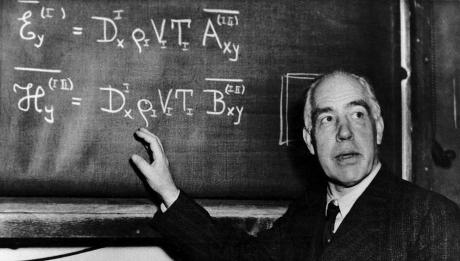
\includegraphics[scale=0.5]{bohr.jpg} \end{centering}

  \bigskip ``Every scientist is constantly confronted with the problem
  of objective description of experience by which we mean
  \textbf{unambiguous communication}.''


  \bigskip ``We must strive continually to extend the scope of our
  description, but in such a way that our messages do not thereby lose
  their \textbf{objective or unambiguous} character.''
\end{frame}

\begin{frame}
  \frametitle{objectivity as univocity}

``\ldots the account of the experimental arrangement and of
  the results of the observations must be expressed in
  \textbf{unambiguous language} with suitable application of the
  terminology of classical physics.''

  \medskip ``\ldots our task must be to account for such experience in
  a manner independent of individual subjective judgment and therefore
  objective in the sense that it can be \textbf{unambiguously
    communicated in ordinary human language}.''

\end{frame}

\begin{frame}
  \frametitle{objectivity as intertranslatability}

  ``The relativistic description is also objective inasmuch as every
  observer can deduce by calculation what the other observer will
  perceive or has perceived.  For all that, we have come a long way
  from the classical ideal of objective descriptions.''

  \bigskip $\Longrightarrow$ bringing harmony to apparently
  disagreeing perceptions

\end{frame}

\begin{frame}
  \frametitle{objectivity as intertranslatability}

  When are two first-order theories $T_1$ and $T_2$ intertranslatable?

  \begin{enumerate}
  \item (Montague) If the relation symbols of $T_1$ can be reinterpreted as
    relations in $T_2$, and the relation symbols of $T_2$ can be
    reinterpreted as relations in $T_1$ such that \dots
  \item (Morita) If the quantifier phrases of $T_1$ can be
    reinterpreted as \dots
  \end{enumerate}


\end{frame}  

\begin{frame}
  \frametitle{standards for good translation}

  \begin{itemize}
  \item Not purely arbitrary \newline
    If arbitrary, then ultimately there are no standards, no truth, no
    good science and bad science  \newline
    Already building upon aeons of shared communication \newline
    Empirical reality is our guide 
  \item Not a simple fact \newline
    Why is this level better than the former? \newline
    The problem of the infinite regress of meta- 
  \end{itemize}
  
\end{frame}


\begin{frame}
  \frametitle{Summary: Bohr on objective description}

  \begin{enumerate}
  \item Objectivity is all about \textbf{unambiguous} communication
  \item Unambiguous communication requires creation of a
    \underline{separation line between subject and object} \newline
    i.e.\ clearly delineating the object of inquiry \newline What
    are we talking about? How does what you're saying play out in
    terms of actions and reactions?
  \item Such a delineation cannot happen at a purely intellectual
    level; it happens through our interactions with the world
    
  \end{enumerate}


\end{frame}



%%%
%%%
%%%

\section{Who is the realist about quantum theory?}

\begin{frame}
\frametitle{The old new story}
  
The Copenhagen (or collapse) interpretation is bad because it involves
an \textbf{observer} as a primitive

\bigskip The many-worlds interpretation is good because it simply
says: the world is like this --- a wavefunction, evolving in time
according to the Schr{\"o}dinger equation

\end{frame}

\begin{frame}
  \frametitle{The new old story}

  The many-worlds interpretation is bad to the extent that it fails to
  tie the relevant mathematical objects (e.g.\ wavefunction) down into
  the shared world of our experience
  
\bigskip To interpret quantum theory is to explain how to use it
(Healey, )

\end{frame}

\begin{frame}
  \frametitle{Lessons}
  \begin{enumerate}
  \item There is no product of scientific activity (e.g.\ theory,
    model) that in itself is objective
  \item There are more or less objective {\it processes of inquiry},
    and {\it modes of communication}
  \item Ironically, the limit of objective description (i.e.\ pure
    math) is again empirically ambiguous \newline ``The world is
    modelled by the number 42!''  \newline ``The world is a four-dimensional
    Lorentzian manifold!''
  \item To communicate unambiguously, one must anchor the description
    in the world of shared experience
  \end{enumerate}
  \end{frame}

\end{document}




%%% Local Variables:
%%% mode: latex
%%% TeX-master: t
%%% End:
